In this section the final system is tested with varying input signal in order to evaluate at what level the application fulfils the practical purpose of the system. According to chapter \ref{ch3} the purpose of the system is to create a spectrogram from which the significant frequencies over time are to be recognized by the peak detection algorithm to match the frequencies known to be in the input signal according to the tone or chord played. \\
In each test the same noise is added to the signal with a maximum SNR at ---- \trine{insæt max SNR}. The noise consists of hands clapping in the background to simulate a realistic situation. Note that all other natural noises are hence minimized. Variation of the noise will not be considered in this system validation but will be further investigated in chapter \ref{ch11}.

\paragraph{Test 1} Scale with clapping hands.
\begin{figure}[H]
\centering
\begin{subfigure}{0.49\textwidth}
\centering
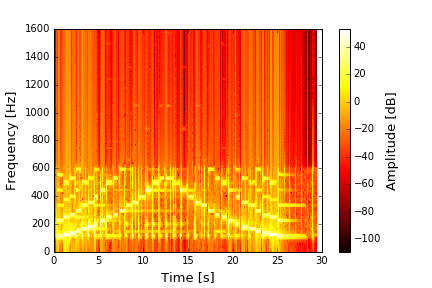
\includegraphics[width=\textwidth]{figures/validation/systemtest/final_spec.png}
\caption{Spectrogram of scale.}
\label{fig:final_spec1}
\end{subfigure}
\begin{subfigure}{0.49\textwidth}
\centering
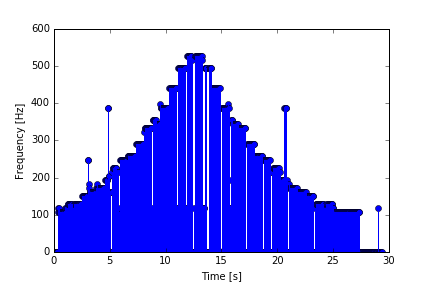
\includegraphics[width=\textwidth]{figures/validation/systemtest/final_peak.png}
\caption{Significant frequencies of scale.}
\label{fig:final_peak1}
\end{subfigure}
\caption{Scale with clapping hands.}
\label{fig:final_1}
\end{figure} 

Figure \ref{fig:final_1} account for the system output of test 1. From the results it is clear that the significant frequencies follows an octatonic scale. However, single incongruous frequencies appears due to a low SNR within the passband at a certain time.
It is clear that the lowest frequencies lay closer as expected, and hence it is a bit harder to identify the actual frequencies. From the result it is concluded that the scale is recognisable.

\paragraph{Test 2} Melody ``Lille Peter edderkop'' by single tones with clapping hands.  
\begin{figure}[H]
\centering
\begin{subfigure}{0.49\textwidth}
\centering
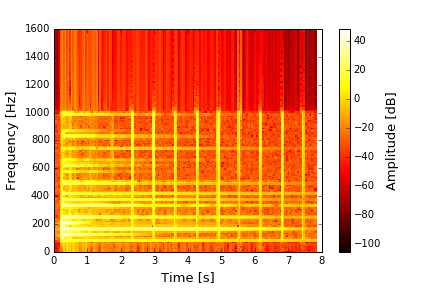
\includegraphics[width=\textwidth]{figures/validation/systemtest/final_spec3.png}
\caption{Spectrogram of melody.}
\label{fig:final_spec2}
\end{subfigure}
\begin{subfigure}{0.49\textwidth}
\centering
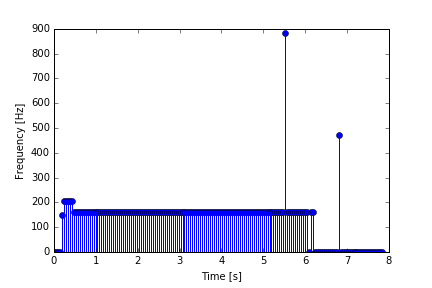
\includegraphics[width=\textwidth]{figures/validation/systemtest/final_peak3.png}
\caption{Significant frequencies of melody.}
\label{fig:final_peak3}
\end{subfigure}
\caption{Melody ``Lille Peter edderkop'' by single tones with clapping hands.}
\label{fig:final_3}
\end{figure}  

Figure \ref{fig:final_3} accounts for the output of test 2. It is seen compared to the result of the scale that the significant frequencies are not as clear due to several incongruous detected frequencies. However, by ignoring the single peaks in figure \ref{fig:final_peak3} it is possible to sense the pattern of the frequencies. The first three different frequencies detected is approximately 258 Hz, 301 Hz and 322 Hz, which corresponds within a range of $\pm 10$ Hz to the first line of the melody being $C \ C \ C \ D \ E \ E \ E$, and it also corresponds with the time axis. More generally, the melody is recognisable by a person knowing the melody. \\
By this one can conclude that the melody is recognisable on behalf of the result but a selective algorithm is required to determine the specific tones.                  

\paragraph{Test 3} Low $E$ chord with clapping hands.
\begin{figure}[H]
\centering
\begin{subfigure}{0.49\textwidth}
\centering
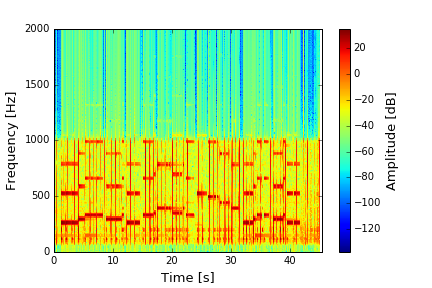
\includegraphics[width=\textwidth]{figures/validation/systemtest/final_spec2.png}
\caption{Spectrogram of $E$ chord.}
\label{fig:final_spec2}
\end{subfigure}
\begin{subfigure}{0.49\textwidth}
\centering
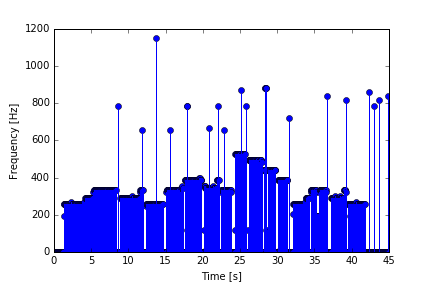
\includegraphics[width=\textwidth]{figures/validation/systemtest/final_peak2.png}
\caption{Significant frequencies of $E$ chord.}
\label{fig:final_peak2}
\end{subfigure}
\caption{Significant frequencies of low $E$ chord.}
\label{fig:final_2}
\end{figure}

Figure \ref{fig:final_2} accounts for the output of test 3. By the detected frequencies shown in figure \label{fig:final_peak2} it seems that it is a single low $E$ tone being played, cf. figure \ref{fig:inte_peak}, rather than the low $E$ chord. As explained in chapter \ref{ch2} a chord is a combination of at least three tones, which in this case is $E$, $B$, $G$\hashsharp and also the harmonics. Hence, the peak detection algorithm is not able to detect chords, and the spectrogram does not provide readable information, neither, because the tones above the significant $E$ tone are difficult to identify. Furthermore, it would require intelligent guessing in order to connect the correct frequencies found to be the most significant. \trine{some one?}

\subsection{Evaluation}
From the test results of the final application it is seen that the system is capable of computing a spectrogram on behalf of a given input signal in form of a .WAW file containing a recorded sound signal. Noise outside a given passband is successfully removed in order to isolate the frequencies expected within the range of significant frequencies of the signal found by the frequency analysis described in chapter \ref{ch9}. \\
From this the implementation of each unit and the integration of these into one algorithm making the application work as intended - technically speaking. \\
\\
Within the limit of the presented theory the quality of the output is sought optimized through the decisions made primarily upon filter type and the resolution of time and frequency, respectively, in the spectrogram.
The quality of the output is evaluated upon the possibility of recognising the correct significant frequency at a specific time. \\
The results of the final tests indicate that it is possible to detect the significant frequency in the case of a single tone within an approximate range of $\pm 10$ Hz. This accuracy is found to be sufficient under the assumption that only the standard tones are used. The exactness in time are not fully obtained but visually it appears sufficient. \\        
Test 1 and test 2 indicates further that when the input signal gets more complicated with respect to speed and shifts between tones it is more difficult to detect the right tones. \\
By test 3 it is concluded that the application is not capable of determining a specific chord. \\   
\\
To summarize, the application is found to fulfil the primary purpose when the input signal is limited to consist of single standard tones recorded under controlled circumstances. \\
The resistance towards varying noise will be investigated in the following chapter.           \trine{skal vi tilføje diskussion om forbedringer? restriktion på filter i forhold til at vi tilpasser?}